\section{Additional Results}
\label{app:additional}

\subsection{All object shapes}
Table~\ref{tab:shape_domains} reports every held-out shape. \ours gives the largest gains on the unseen shapes: with GD, I rises from 44.7\% (AdaJEPA) to 77.6\% and square from 46.7\% to 61.1\%. It also leads on the seen shapes in aggregate.

\begin{table*}[t]
 \centering
 \caption{Held-out success (\%) per PushObj shape. I, square, and small tee are unseen in pretraining. All averages the seven shapes.}
 \label{tab:shape_domains}
 \small
 \begin{tabular}{llcccccccc}
 \toprule
 Planner & Method & I & L & Square & Z & Small tee & Plus & T & All\\
 \midrule
 \inputrows{tables/shape_domains.tex}
 \bottomrule
 \end{tabular}
\end{table*}

\subsection{All visual conditions}
Table~\ref{tab:visual_domains} and Fig.~\ref{fig:visual_gains} break the paired visual results down by condition. \ours improves on all seven conditions with both planners. The largest gains, more than 25 points, appear under red-object and red-goal recoloring, where episodic adaptation has to rediscover the new appearance in every episode.

\begin{table*}[t]
 \centering
 \caption{Held-out visual success (\%) per condition on the paired targets. All averages seven conditions; Shift excludes Original.}
 \label{tab:visual_domains}
 \small
 \begin{tabular}{llccccccccc}
 \toprule
 Planner & Method & Original & Blur & Noise & Dark & Red agent & Red object & Red goal & All & Shift\\
 \midrule
 \inputrows{tables/visual_domains.tex}
 \bottomrule
 \end{tabular}
\end{table*}

\begin{figure*}[t]
 \centering
 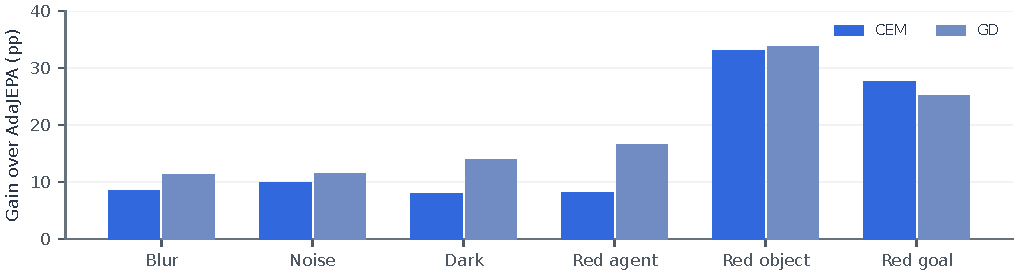
\includegraphics[width=\textwidth]{visual_gains.pdf}
 \caption{Held-out gain of \textbf{\ours} over AdaJEPA for each visual shift, in percentage points.}
 \label{fig:visual_gains}
\end{figure*}

\subsection{Planning efficiency}
Figure~\mainref{fig:efficiency_main} plots cumulative held-out success against the number of MPC replans. \ours pulls ahead within the first four replans and keeps the lead for the rest of the budget, showing how the advantage develops before the final 30-replan evaluation.



\subsection{Deformable manipulation}


Figure~\mainref{fig:deployment} shows the four-pass learning curves in the main paper. Table~\ref{tab:deform} adds standard errors to the deformable results of Table~\mainref{tab:main}. Table~\ref{tab:deform_passes} follows consolidation pass by pass at two slow learning rates. With $10^{-4}$, CD decreases at every pass on both tasks. With $2\times10^{-4}$, rope improves faster in the early passes and both rates reach a similar level after four passes, so consolidation is robust to the learning rate.

\begin{table}[t]
  \centering
  \caption{Deformable manipulation: mean CD $\pm$ standard error over 50 instances. \ours uses its slow predictor after four passes.}
  \label{tab:deform}
  \small
  \begin{tabular}{lcc}
    \toprule
    Method & Rope CD $\downarrow$ & Granular CD $\downarrow$\\
    \midrule
    \inputrows{tables/deform_rows.tex}
    \bottomrule
  \end{tabular}
\end{table}

\begin{table}[t]
  \centering
  \caption{CD of \ours after each consolidation pass at two slow learning rates (mean $\pm$ standard error, 50 instances).}
  \label{tab:deform_passes}
  \footnotesize
  \setlength{\tabcolsep}{2.5pt}
  \begin{tabular}{ccccc}
    \toprule
    & \multicolumn{2}{c}{lr $10^{-4}$} & \multicolumn{2}{c}{lr $2\times10^{-4}$}\\
    \cmidrule(lr){2-3}\cmidrule(lr){4-5}
    Pass & Rope & Granular & Rope & Granular\\
    \midrule
    \inputrows{tables/deform_passes.tex}
    \bottomrule
  \end{tabular}
\end{table}

\subsection{A seven-round shape stream}
A second PushObj stream runs seven rounds with a slow learning rate of $2\times10^{-4}$, one chain per planner. Each round has 50 episodes per shape, drawn without replacement and excluding the held-out sources, for 2{,}450 episodes per planner. Online success rises from 70.6\% in the first round to 78.6\% in the seventh with GD, and from 72.3\% to 78.3\% with CEM.

The episode logs record the fast-update fingerprint of every episode. Figure~\ref{fig:directions} shows the cosine between consecutive fingerprints: the mean is 0.018 for both planners, and most of the mass lies near zero. These measurements support consolidating transition data rather than accumulating episode-specific parameter updates (Sec.~\mainref{sec:diagnosis}). Over the stream, \ours writes 622 (GD) and 663 (CEM) episodes to memory, 25.4\% and 27.1\% of all episodes, and finishes 630 and 666 episodes with a slow predictor.

\begin{figure*}[t]
 \centering
 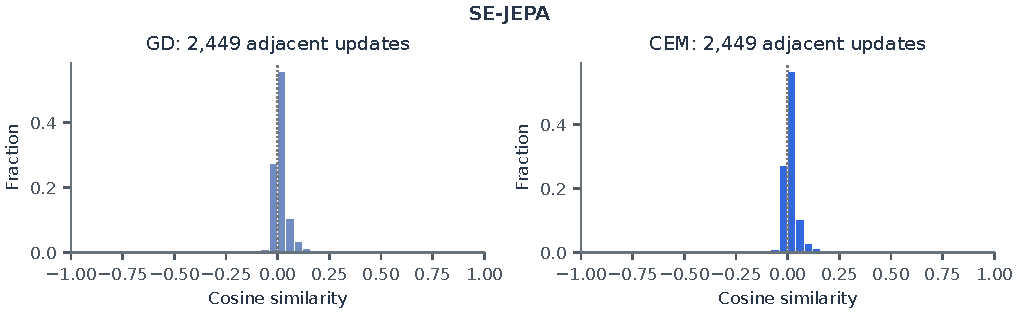
\includegraphics[width=\textwidth]{update_directions.pdf}
 \caption{Cosine similarity between consecutive fast-update fingerprints in the seven-round shape stream (2{,}449 pairs per planner).}
 \label{fig:directions}
\end{figure*}

\subsection{What \ours chooses to learn}
\label{sec:selectivity}

\ours learns selectively. In a seven-round PushObj stream of 2{,}450 episodes per planner, it writes only 25\% (GD) to 27\% (CEM) of episodes to memory; the rest are familiar to the pretrained model, still pending, or rejected by validation. Retrieval is just as targeted: slow predictors plan about one episode in four, and the reference handles the rest.

Selective writing leaves familiar dynamics to the pretrained model, which \ours never overwrites. On the four pretraining shapes, \ours reaches 86.0\% held-out success with CEM and 88.4\% with GD, against 82.3\% and 84.8\% for AdaJEPA. This preserves a useful pretrained reference while allowing specialized predictors to add capacity for recurring shifts.
